\chapter{Lindenmayer-Systeme} \label{ch:LSysteme}

In diesem Kapitel werden Regeln für die Definition von Lindenmayer-Systemen -- kurz: L-Systemen -- festgelegt und die verwendete Methode zur Visualisierung der Ergebnisse von L-Systemen besprochen. Es findet eine Beschränkung des Themas auf die in dieser Arbeit umgesetzten Konzepte statt.

\section{Kontextfreie Grammatik}

Bei L-Systemen handelt es sich um auf Zeichenketten basierende Ersetzungssysteme. Es werden komplexe Objekte beschrieben, indem Teile der Zeichenkette durch andere Zeichen oder Zeichenketten ersetzt werden. Die Beschreibung dieser Ersetzungen findet mittels festgelegter Produktionsregeln statt. \cite[S.2]{ABOP:04} 

Eine formale Definition eines auf Zeichenketten arbeitenden Ersetzungssystems wird durch kontextfreie Grammatiken gegeben:

\newtheorem{defKontextfreieGrammatik}{Kontextfreie Grammatik:}[chapter]
\begin{defKontextfreieGrammatik}
	Eine kontextfreie Grammatik G ist ein Tupel G = $(V, N, P, \omega)$ bestehend aus:
	
	\begin{description}[labelindent]
		\item[\boldmath$V$] Einer nichtleeren, endlichen Menge von Buchstaben (Alphabet).\\
		
		\item[\boldmath$N$] Einer endlichen Menge von Variablen.\\
		
		\item[\boldmath$P$] Einer endlichen Menge von Produktionsregeln in der Form $P: A \rightarrow \alpha$ mit $A \in N$ und $\alpha \in (V \cup N )^*$.\\
		
		\item[\boldmath$\omega \in N$] Dem Axiom, Startsymbol der Grammatik.\\
		
	\end{description}
	\cite[S.343]{ThI:14}
\end{defKontextfreieGrammatik}

Die Menge $V^*$ ist die Menge aller Wörter über $V$, d.h. die Menge aller Wörter, die aus dem Alphabet $V$ gebildet werden können. \cite[S.70]{ThI:14} 

Eine Grammatik wird als kontextfrei bezeichnet, wenn beispielsweise die Produktionsregel $A \rightarrow \alpha$ angewendet werden kann, ohne die $A$ umgebenden Buchstaben -- seinen Kontext -- beachten zu müssen. \cite[S.343]{ThI:14} 

Eine Grammatik wird als deterministisch bezeichnet, wenn es genau eine Produktionsregel $r \in P$ für jede Variable $A \in N$ gibt, sodass $r: A \rightarrow \alpha$, $\alpha \in (V \cup N )^*$. Das bedeutet, dass die Ersetzung einer Variable eindeutig durch eine einzige Regel beschrieben wird. \cite[S.75]{PCGiG:16}

Die Anwendung der Produktionsregeln findet meist sequentiell statt -- die Zeichenkette wird von links nach rechts durchlaufen und Ersetzungen werden direkt auf die untersuchte Zeichenkette angewendet. \cite[S.75]{PCGiG:16}

\section{D0L-Systeme}

Diese Arbeit beschränkt sich auf die Behandlung deterministischer, kontextfreier L-Systeme, auch D0L-Systeme genannt. Diese besitzen die Eigenschaften einer deterministischen und kontextfreien Grammatik, Produktionsregeln werden jedoch parallel und gleichzeitig auf alle Buchstaben des untersuchten Wortes angewendet. Dieses Vorgehen soll die Zellteilung in mehrzelligen Organismen simulieren und ist somit an biologische Vorgänge angelehnt. \cite[S. 3]{ABOP:04} 

Ein D0L-System kann wie folgt definiert werden:
\newtheorem{defD0LSystem}{D0L-System:}[chapter]
\begin{defD0LSystem}
	Ein D0L-System ist ein Tupel G = $(V, P, \omega)$, bestehend aus:
	
	\begin{description}[labelindent]
		\item[\boldmath$V$] Einem nichtleeren, endlichen Alphabet.\\
		
		\item[\boldmath$P$] Einer endlichen Menge von Produktionsregeln in der Form $P: a \rightarrow b$ mit $a \in V$ und $b \in V^*$. $a$ wird als Vorgänger, $b$ als Nachfolger bezeichnet. Ist für einen Buchstaben $x \in V$ keine explizite Produktionsregel angegeben, wird die Identitätsproduktion $P: x \rightarrow x$ angenommen -- der Buchstabe wird durch sich selbst ersetzt.\\
		
		\item[\boldmath$\omega \in V^+$]  Dem Axiom, Startsymbol der Grammatik.		
	\end{description}
\cite[S.4]{ABOP:04} 
\end{defD0LSystem}
Die Menge $V^+$ ist die Menge aller nichtleeren Wörter über $V$.  

Die Ableitung eines Wortes entspricht der Ersetzung aller Buchstaben anhand der Produktionsregeln. Ein Wort kann mehrmals abgeleitet werden. 

\newtheorem{defAbleitung}{Ableitung:}[chapter]
\begin{defAbleitung}
	Gegeben sei ein Wort $w = a_1 ... a_m$ mit $w \in V^*$ und $a_i \in V^*$. Das Wort $v = b_1 ... b_m$ mit $v \in V^*$ und $b_i \in V^*$ ist die Ableitung von $w$ wenn für alle $i=1...m$ eine Produktionsregel $a_i \rightarrow b_i$ existiert. Die Ableitung wird als $w \Rightarrow v$ notiert. \\
	Das Wort $w_n$ ist die n-te Ableitung des Wortes $w_0$ wenn eine Folge von Wörtern $w_0, w_1, ..., w_n$ mit Ableitungen $w_0 \Rightarrow w_1 \Rightarrow ... \Rightarrow w_n$ existiert. \cite[S.4]{ABOP:04} 
\end{defAbleitung}


Beispiel: Das Wachstum der Blaualgen-Gattung \glqq Anabaena\grqq{} kann durch ein L-System simuliert werden. Die Buchstaben $a$ und $b$ beschreiben die Größe und Teilungsbereitschaft einer Algenzelle, während die Indizes $l$ und $r$ die Polarität einer Zelle darstellen. Es gelten folgende Produktionsregeln:
\begin{equation}
\begin{array}{cccc}
 p_1 & : a_r &\rightarrow& a_lb_r \\
p_2 &  : a_l &\rightarrow& b_la_r \\ 
p_3 &  : b_r &\rightarrow& a_r \\
p_4 &  : b_l &\rightarrow& a_l 
\end{array}
\label{eq:ProdAnabaena}
\end{equation} 

Die Entwicklung einer Anfangszelle $a_r$ (Axiom $\omega : a_r$) läuft daraufhin wie in Abbildung \ref{fig:AnabaenaAbleitung} dargestellt ab.
\begin{figure} [hbtp]
	\centering
	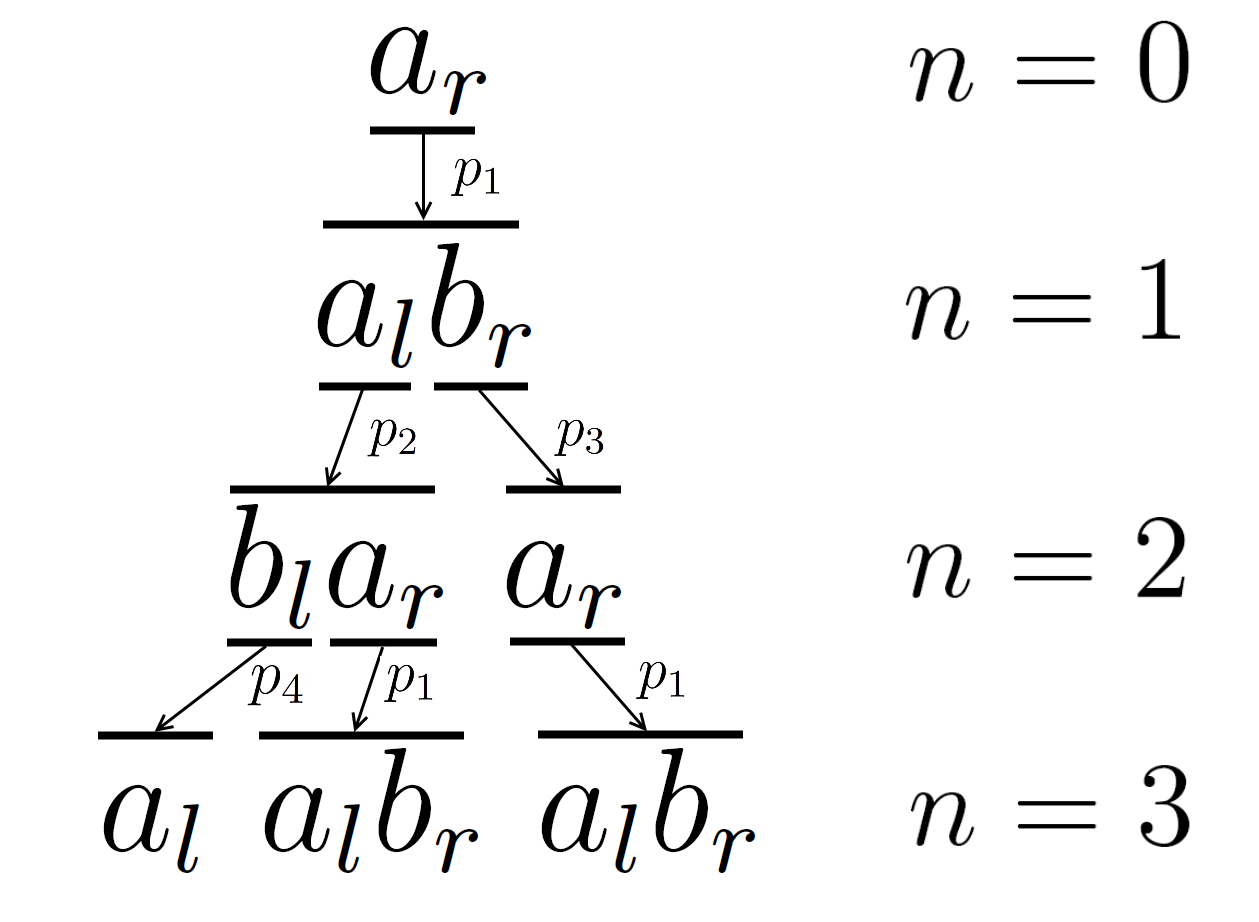
\includegraphics[height=0.25\textheight]{images/AnabaenaAbleitung.png}
	\caption{Die n-fache Ableitung der Anfangszelle $a_r$ anhand der Produktionsregeln $p_1 ... p_4$ aus Gleichung \ref{eq:ProdAnabaena}. Eigene Abbildung auf Grundlage von \cite[S.4]{ABOP:04}.}
	\label{fig:AnabaenaAbleitung}
\end{figure}

\subsection{Parametrische L-Systeme}

Parametrische L-Systeme stellen eine Erweiterung der D0L-Systeme dar. Die Buchstaben eines verwendeten Alphabets $V$ werden um zugeordnete Parameter aus der Menge der reellen Zahlen ergänzt. Ein solches parametrisches Wort $V \times \mathbb{R}^*$ besteht aus einem Zeichen $A \in V$ und Parametern $a_1,...,a_n \in \mathbb{R}$ und wird als $A(a_1,...,a_n)$ dargestellt. Ein parametrisches Wort ohne Parameter mit dem Zeichen $A \in V$  wird schlicht als $A$ dargestellt. \cite[S.41]{ABOP:04}

Die obige Definition von parametrischen Worten geschieht mithilfe von numerischen Konstanten, während bei der Angabe eines L-Systems formale Parameter verwendet werden. Im informatischen Kontext entspricht der Begriff eines formalen Parameters einem Funktionsparameter oder Funktionsvariablen. \cite[S.16f]{FormalParamDef:05} Ist $\Sigma$ eine Menge von formalen Parametern, dann ist $E(\Sigma)$ ein arithmetischer Ausdruck, in dem Parameter, Konstanten und arithmetische Operatoren auf eine zulässige Weise kombiniert werden. \cite[S.41]{ABOP:04}

\newtheorem{defParametrischeLSysteme}{Parametrisches L-System:}[section]
\begin{defParametrischeLSysteme}
	Ein Parametrisches L-System ist ein Tupel G = $(V, \Sigma, P, \omega)$, bestehend aus:
	\begin{description}[labelindent]
		\item[\boldmath$V$] Einem nichtleeren, endlichen Alphabet.\\
		
		\item[\boldmath$\Sigma$] Einer Menge von formalen Parametern.\\
		
		\item[\boldmath$P$] Einer endlichen Menge von Produktionsregeln $P : (V\times \Sigma^*) \rightarrow (V\times E(\Sigma))^*$\\
		
		\item[\boldmath$\omega \in M^+$] mit $M =(V \times \mathbb{R}^*)$ -- einem Axiom in Form eines nichtleeren, parametrischen Wortes.
	\end{description}
\cite[S.41]{ABOP:04}
\end{defParametrischeLSysteme}

Eine Produktionsregel kann auf ein parametrisches Wort angewendet werden wenn das Zeichen, welches dem Wort vorausgeht, und die Anzahl der Parameter mit dem Zeichen und der Parameteranzahl im Vorgänger der Produktionsregel übereinstimmen. \cite[S.42]{ABOP:04}

Beispiel: Gegeben sei folgendes, parametrisches L-System:

\begin{equation}
\begin{array}{llll}
\omega & : A(1,1) \\
p_1 & : A(x,y) &\rightarrow& A(x+1, y*2)\text{ }B(y) \\
p_2 &  : B(x) &\rightarrow& B(x+1)\text{ }C 
\end{array}
\label{eq:ProdParamLSystem}
\end{equation} 

Das Alphabet $V$ und die Menge der formalen Parameter $\Sigma$ gehen implizit aus der Angabe der Produktionsregeln hervor und werden in zukünftigen L-System-Gleichungen nicht angegeben. Die Entwicklung des L-Systems läuft wie in Abbildung \ref{fig:ParamLSystemBeispiel} gezeigt ab. 

\begin{figure} [hbtp]
	\centering
	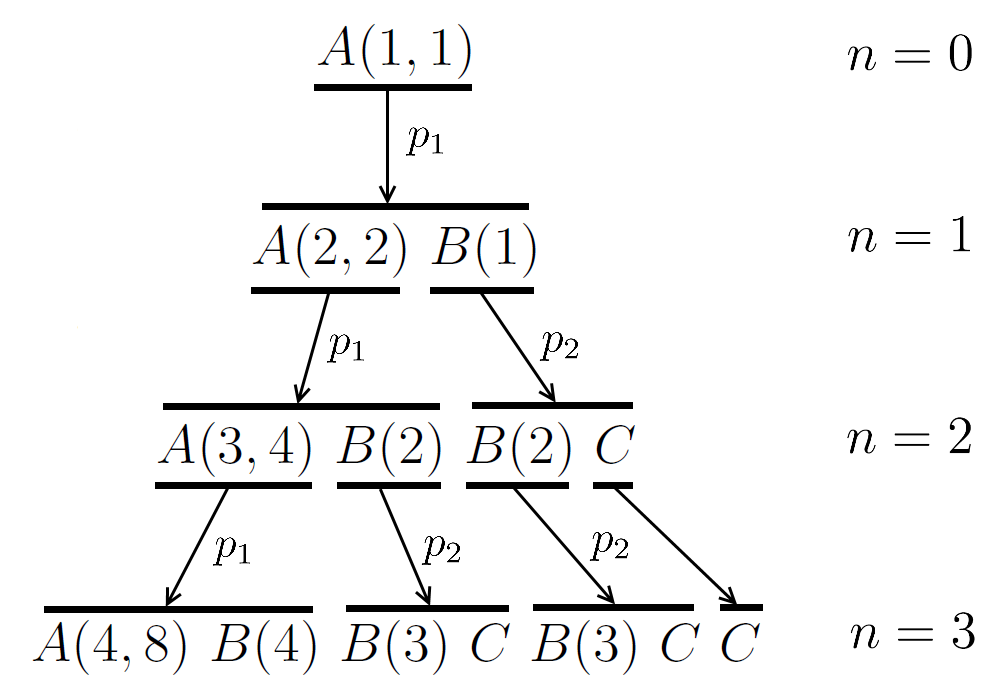
\includegraphics[height=0.3\textheight]{images/ParamLSystemBeispiel.png}
	\caption{Die n-fache Ableitung des Axioms $A(1,1)$ anhand der Produktionsregeln aus Gleichung \ref{eq:ProdParamLSystem}. Die Ersetzung des Zeichens $C$ erfolgt anhand der impliziten Identitätsproduktion. Eigene Abbildung.}
	\label{fig:ParamLSystemBeispiel}
\end{figure}

\section{Grafische Interpretation von L-Systemen}

Um die Ergebnisse von L-Systemen in Form von dreidimensionalen Objekten zu visualisieren, muss eine grafische Interpretation der resultierenden Zeichenketten festgelegt werden. Im Folgenden wird die verwendete Visualisierungsmethode -- die Turtle-Interpretation -- vorgestellt.

\subsection{Turtle-Interpretation}

Die Turtle-Interpretation im zweidimensionalen Raum entspricht der Vorstellung einer Turtle (engl. für Schildkröte) auf einem Blatt Papier. Die Turtle besitzt eine Position $\overrightarrow{p}$ sowie einen Einheitsvektor $\overrightarrow{H}$ in kartesischen Koordinaten. $\overrightarrow{p}$ beschreibt die Position der Turtle auf der Ebene und $\overrightarrow{H}$ entspricht der Blickrichtung (Heading) der Turtle. Der Zustand einer Turtle wird somit vollständig durch die Position und Blickrichtung definiert und wird als Tupel $(\overrightarrow{p},\overrightarrow{H})$ angegeben. \cite[S.2]{Turtle:04} Die Ausgangsposition entspricht dem Ursprung des lokalen Koordinatensystems der Turtle. 

Es können drei Aktionen durchführt werden, welche durch die folgenden Symbole dargestellt werden:

\begin{description}[labelindent]
	\item[\boldmath$F(l)$] Die Turtle bewegt sich um $l>0$ in die Richtung der aktuellen Blickrichtung. Die neue Position ist  $\overrightarrow{p_{neu}}$ mit:
	\begin{equation}
	\begin{array}{ll}
	\overrightarrow{p_{neu}} & = \overrightarrow{p} + \overrightarrow{H} * l
	\end{array}
	\end{equation} 
	Zwischen der alten Position $\overrightarrow{p}$ und der neuen Position $\overrightarrow{p_{neu}}$ wird eine Linie gezeichnet.\\
	
	\item[\boldmath$+(d)$]  Die Turtle dreht sich um den Winkel $d$ nach links. Die neue Blickrichtung ist $\overrightarrow{H'}$ mit:
	\begin{equation}
	\overrightarrow{H'} = 
	\setlength\arraycolsep{10pt}
	\begin{pmatrix}
	cos(d) & -sin(d)\\
	sin(d) & cos(d)
	\end{pmatrix}
	* \overrightarrow{H}
	\end{equation} 
	
	\item[\boldmath$-(d)$]  Die Turtle dreht sich um den Winkel $d$ nach rechts. Die neue Blickrichtung ist $\overrightarrow{H'}$ mit:
	\begin{equation}
	\overrightarrow{H'} = 
	\setlength\arraycolsep{10pt}
	\begin{pmatrix}
	cos(d) & sin(d)\\
	-sin(d) & cos(d)
	\end{pmatrix}
	* \overrightarrow{H}
	\end{equation} 
	
\end{description}
\cite[S.4,46]{Turtle:04} \cite[S.7]{ABOP:04}
Die Symbole \glqq+\grqq{} und \glqq-\grqq{} werden sowohl im Alphabet eines L-Systems als auch bei arithmetischen Operationen in Parameterangaben verwendet, ihre Bedeutung ist abhängig vom Kontext, in dem sie angewendet werden. \cite[S.46]{ABOP:04}

Die grafische Turtle-Interpretation einer Zeichenkette, die durch ein L-System zurückgegeben wird, sind somit die Linien, die auf Grundlage der definierten Symbole gezeichnet werden. 

Beispiel: Mithilfe von L-Systemen und einer Turtle-Interpretation können Fraktale, in diesem Beispiel sogenannte Koch-Kurven, visualisiert werden. Diese Kurven bestehen aus einem Initiator -- einer einfachen, zweidimensionalen Form -- und einem Generator, der einem offenen Polygonzug entspricht. In jedem Ableitungsschritt, angefangen bei dem Initiator, wird jede gerade Linie durch den Generator ersetzt. \cite[S.39]{Mandelbrot:16} 

\begin{figure} [hbtp]
	\centering
	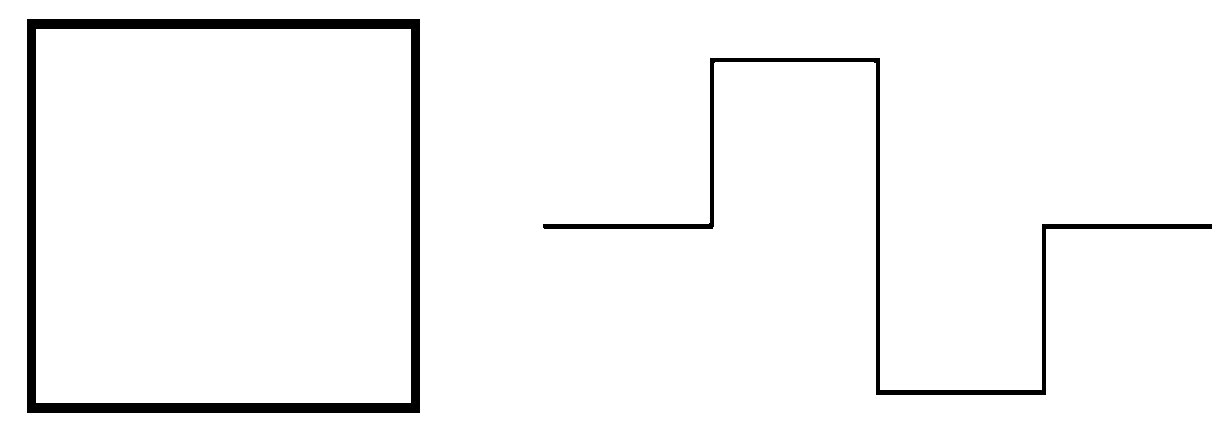
\includegraphics[width=0.6\textwidth]{images/InitiatorGenerator.png}
	\caption{Links: Initiator der Koch-Kurve in Form eines einfachen Quadrats. Rechts: Generator der Koch-Kurve in Form eines offenen Polygonzugs. Eigene Abbildungen.}
	\label{fig:InitiatorGenerator}
\end{figure}

Dieses Verhalten kann nun auf ein L-System abgebildet werden: Der Initiator entspricht dem Axiom und der Generator einer Produktionsregel des L-Systems. Der in Abbildung \ref{fig:InitiatorGenerator} dargestellte Initiator und Generator entsprechen der Turtle-Interpretation des folgenden L-Systems:

\begin{equation}
\begin{array}{llll}
\omega & : F-F-F-F \\
p_1 & : F \rightarrow F+F-F-FF+F+F-F
\end{array}
\label{eq:ProdKochKurve}
\end{equation} 

Für eine bessere Übersicht wurde die Angabe der Parameter weggelassen. Die Turtle interpretiert $F$ als $F(l)$, $-$ als $-(d)$ und $+$ als $+(d)$ mit festgelegter Strichlänge $l$ und Drehwinkel $d$. \label{desc:TurtleWithoutParams} Die Entwicklung des L-Systems läuft, als Turtle-Interpretation visualisiert, wie in Abbildung \ref{fig:KochkurveAbleitung} dargestellt ab.

\begin{figure} [hbtp]
	\centering
	\begin{subfigure}[t]{.4\textwidth}
		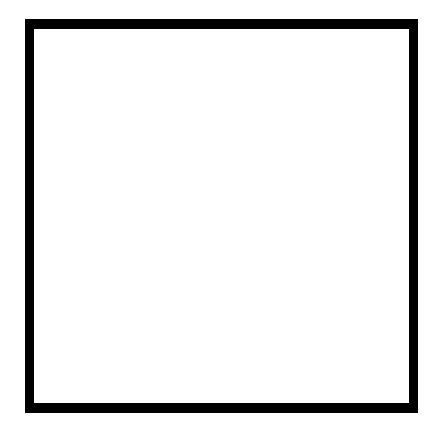
\includegraphics[width=\linewidth]{images/KochkurveN0L400.png}
		\caption{$n=0$, $l=400$, $d=90\degree$}
		\label{fig:KochkurveN0L400}
	\end{subfigure}
	\hspace{.1\textwidth}
	\begin{subfigure}[t]{.4\textwidth}
		\centering
		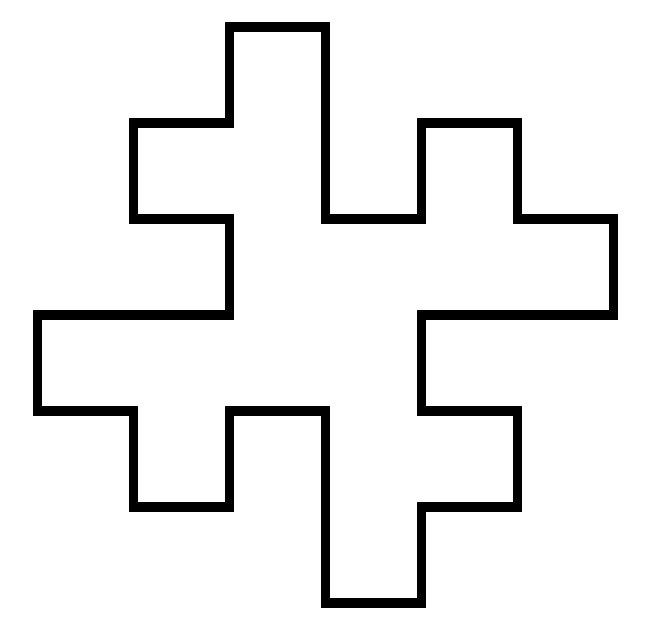
\includegraphics[width=\linewidth]{images/KochkurveN1L100.png}
		\caption{$n=1$, $l=100$, $d=90\degree$}
		\label{fig:KochkurveN1L100}
	\end{subfigure}
	\medskip
	\begin{subfigure}[t]{.4\textwidth}
		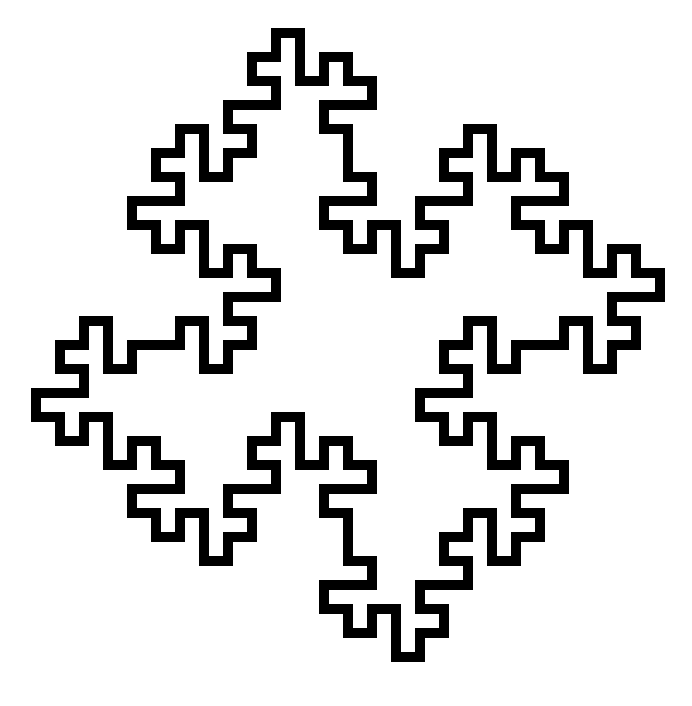
\includegraphics[width=\linewidth]{images/KochkurveN2L25.png}
		\caption{$n=2$, $l=25$, $d=90\degree$}
		\label{fig:KochkurveN2L25}
	\end{subfigure}
	\hspace{.1\textwidth}
	\begin{subfigure}[t]{.4\textwidth}
		\centering
		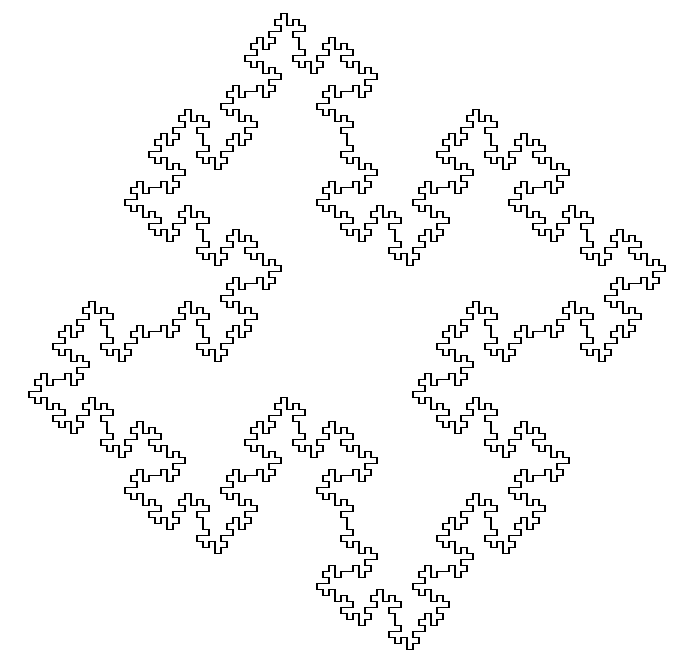
\includegraphics[width=\linewidth]{images/KochkurveN3L6_25.png}
		\caption{$n=3$, $l=6.25$, $d=90\degree$}
		\label{fig:KochkurveN3L6_25}
	\end{subfigure}
	\caption{Die n-fache Ableitung des Axioms $\omega$ anhand der Produktionsregel $p_1$ aus Gleichung \ref{eq:ProdKochKurve}, visualisiert mithilfe der implementierten Turtle-Interpretation. Eigene Abbildungen.}
	\label{fig:KochkurveAbleitung}
\end{figure}

\subsection{Verzweigte L-Systeme} \label{subsec:BranchingLSystems}

Die bisherigen Definitionen von L-Systemen und die korrespondierende Turtle-Interpretation lässt lediglich die Bildung von Grafiken zu, die einen einzelnen, zusammenhängenden Polygonzug erlauben. Um L-Systeme zu bilden, deren Visualisierungen Baumstrukturen ähneln, muss die bisherige Turtle-Interpretation um die Möglichkeit erweitert werden Verzweigungen zu verarbeiten. \cite[S.24]{ABOP:04} 

Folgende Operationen werden eingeführt:

\begin{description}[labelindent]
	\item[\textbf{[}] Der aktuelle Zustand der Turtle in Form ihrer Position und Rotation wird auf einem Stack (engl. für Kellerspeicher) abgelegt. \cite[S.24]{ABOP:04} \\
	
	\item[\textbf{]}] Der oberste Zustand der Turtle wird vom Stack genommen. Die aktuelle Position und Rotation der Turtle wird auf die im Zustand gespeicherte Position und Rotation gesetzt. Es wird keine Linie zwischen der alten und neuen Position gezeichnet. \cite[S.24]{ABOP:04} 
\end{description}

Diese Erweiterung erlaubt es mehrere Linien zu zeichnen, die von einem einzigen Punkt ausgehen -- die Visualisierung von Abzweigungen ist somit möglich. Die Operatoren \textbf{[} und \textbf{]} markieren den Anfang und das Ende eines Zweiges. \cite[S.24]{ABOP:04} 

Beispiel: Mithilfe von verzweigten L-System-Beschreibungen lassen sich die in Abbildung \ref{fig:BranchingLSystems} gezeigten Strukturen bilden. Die Turtle-Interpretation folgt der in \ref{desc:TurtleWithoutParams} beschriebenen Interpretation mit fester Strichlänge $l$ und festem Drehwinkel $d$.

\begin{figure} [hbtp]
	\centering
	\begin{subfigure}[t]{.4\textwidth}
		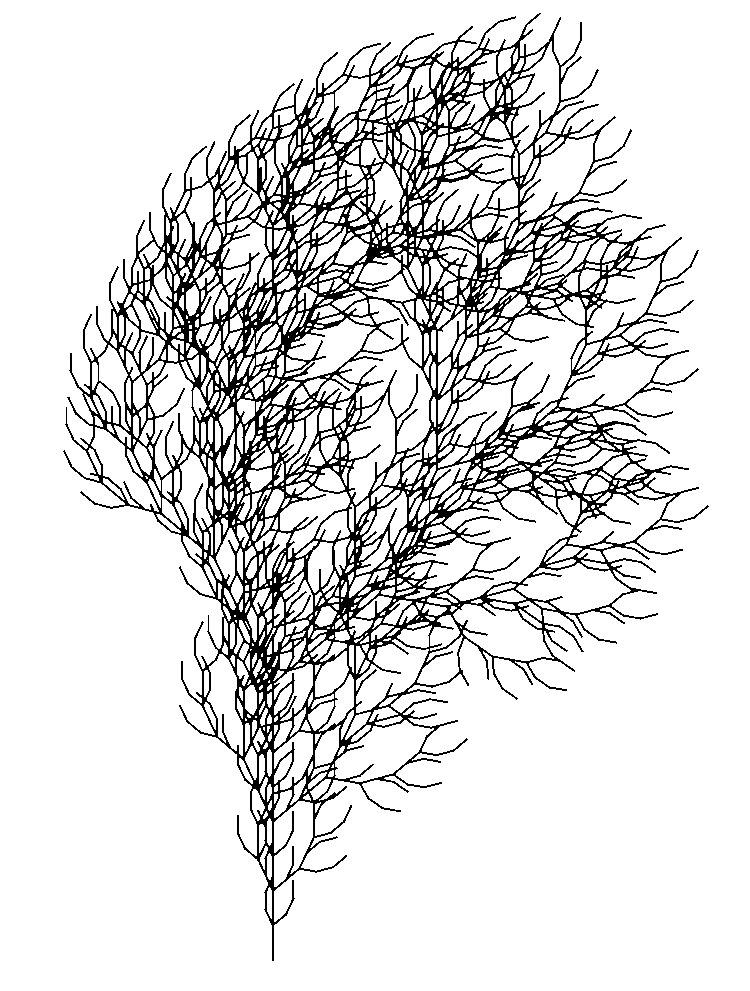
\includegraphics[width=\linewidth]{images/Branching1_N4L18D25.png}
		\caption{$n=4$, $l=18$, $d=25\degree$\\ \\
			$\begin{array}{ll}
				\omega & : F \\
				p_1 & : F \rightarrow FF-[-F+F+F]+[+F-F-F]
			\end{array}
			\label{eq:ProdBranching1}$\\
			\cite[S.25]{ABOP:04}
		}
		\label{fig:Branching1L18D25}
	\end{subfigure}
	\hspace{.15\textwidth}
	\begin{subfigure}[t]{.4\textwidth}
		\centering
		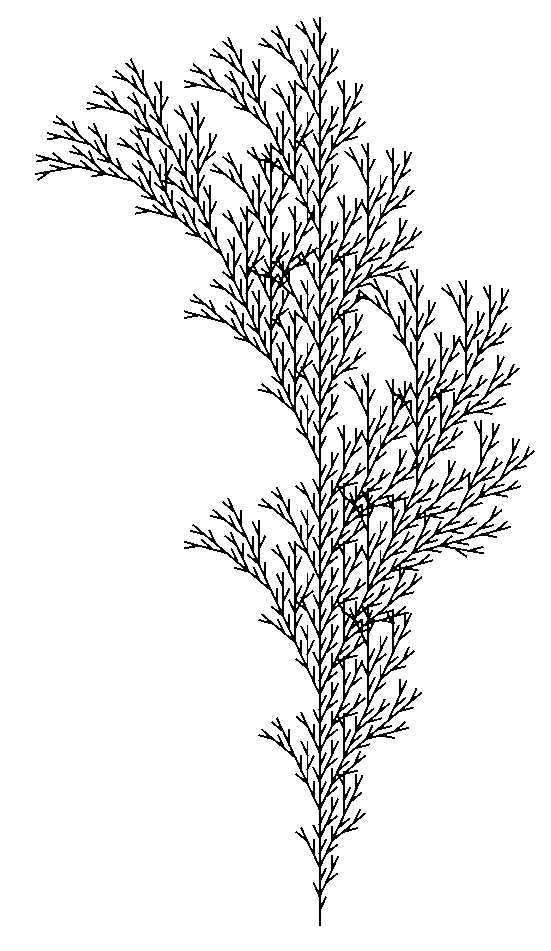
\includegraphics[width=\linewidth]{images/Branching2_N5L15D25.png}
		\caption{$n=5$, $l=15$, $d=25\degree$\\ \\
			$\begin{array}{ll}
				\omega & : F \\
				p_1 & : F \rightarrow F[-F]F[+F][F]
			\end{array}
			\label{eq:ProdBranching2}$\\
			\cite[S.78]{PCGiG:16}
		}
		\label{fig:Branching2L15D25}
	\end{subfigure}

	\caption{Die n-fache Ableitung der Axiome anhand der Produktionsregeln, visualisiert mithilfe der implementierten Turtle-Interpretation. Eigene Abbildung.}
	\label{fig:BranchingLSystems}
\end{figure}

\subsection{Erweiterung der Turtle-Interpretation in den dreidimensionalen Raum}

Die bisherige Definition eines Turtle-Zustands mithilfe einer zweidimensionalen Position und einer Blickrichtung genügt nicht, um Visualisierungen von L-Systemen in Form von dreidimensionalen Baumstrukturen zu ermöglichen. Sowohl die Zustands-Definition als auch die interpretierten Operationen müssen angepasst und erweitert werden.

Der Zustand der Turtle im dreidimensionalen Raum besitzt eine Position $\overrightarrow{p}$ sowie eine $3\times3$ Rotationsmatrix $\boldsymbol{R}$, welche die Orientierung der Turtle im Raum beschreibt. Der Zustand wird als Tupel $(\overrightarrow{p}, \boldsymbol{R})$ angegeben. $\boldsymbol{R}$ entspricht zu Anfang einer Identitätsmatrix. Die Einheitsvektoren $H$, $L$ und $U$  sind orthogonal zueinander und bilden das lokale Koordinatensystem der Turtle. 

\begin{description}[labelindent]
		\item[\boldmath$\overrightarrow{H}$]Die Blickrichtung (Heading-Vektor) der Turtle. Eine Rotation um diesen Vektor um den Winkel $d$ entspricht der Rotationsmatrix $R_{\overrightarrow{H}}$:\\
		\begin{equation}
		R_{\overrightarrow{H}}(d) = 
		\setlength\arraycolsep{10pt}
		\begin{pmatrix}
		1	 	& 0			& 0 \\
		0		& cos(d)	& sin(d) \\
		0 		& -sin(d)	& cos(d)
		\end{pmatrix}	
		\label{eq:rotH}
		\end{equation} 
		
		\item[\boldmath$\overrightarrow{L}$] Der Vektor, der im lokalen Koordinatensystem der Turtle nach links zeigt (Left-Vektor). Eine Rotation um diesen Vektor um den Winkel $d$ entspricht der Rotationsmatrix $R_{\overrightarrow{L}}$:\\
		\begin{equation}
		R_{\overrightarrow{L}}(d) = 
		\setlength\arraycolsep{10pt}
		\begin{pmatrix}
		cos(d) 	& 0		 	& sin(d) \\
		0		& 1			& 0 \\
		-sin(d)	& 0 		&  cos(d)
		\end{pmatrix}	
		\label{eq:rotL}
		\end{equation} 
		
		\item[\boldmath$\overrightarrow{U}$]Der Vektor, der im lokalen Koordinatensystem der Turtle nach oben zeigt (Up-Vektor). Eine Rotation um diesen Vektor um den Winkel $d$ entspricht der Rotationsmatrix $R_{\overrightarrow{U}}$:\\
		\begin{equation}
		R_{\overrightarrow{U}}(d) = 
		\setlength\arraycolsep{10pt}
		\begin{pmatrix}
		cos(d) 	& -sin(d) 	& 0 \\
		sin(d)	& cos(d) 	& 0 \\
		0 		& 0 		& 1
		\end{pmatrix}	
		\label{eq:rotU}
		\end{equation} 
		
	
\end{description}
\cite[S.19]{ABOP:04} \cite[S.69]{Deussen:05} \\

Die erweiterte Turtle-Interpretation verarbeitet folgende Symbole:

\begin{description}[labelindent]
	\item[\boldmath$F(l)$]  Die Turtle bewegt sich um $l>0$ in Blickrichtung $\overrightarrow{H}$. Die neue Position ist $\overrightarrow{p_{neu}}$ mit:
	\begin{equation}
	\begin{array}{ll}
	\overrightarrow{p_{neu}} & = \overrightarrow{p} + \boldsymbol{R} * \overrightarrow{H} * l
	\end{array}
	\label{eq:Turtle3D_F}
	\end{equation} 
	Zwischen der alten Position $p$ und der neuen Position $p_{neu}$ wird eine Linie gezeichnet. \\
	
	\item[\boldmath$+(d)$]  Die Turtle dreht sich nach links um den Winkel $d$. Die neue Rotationsmatrix entspricht $\boldsymbol{R'}$ mit:\\
	\begin{equation}
	\begin{array}{ll}
	\boldsymbol{R'} & =  \boldsymbol{R} * R_{\overrightarrow{U}}(d)
	\end{array}
	\end{equation} 
	
	\item[\boldmath$-(d)$]  Die Turtle dreht sich nach rechts um den Winkel $d$. Die neue Rotationsmatrix entspricht $\boldsymbol{R'}$ mit:\\
	\begin{equation}
	\begin{array}{ll}
	\boldsymbol{R'} & =  \boldsymbol{R} * R_{\overrightarrow{U}}(-d)
	\end{array}
	\end{equation} 
	
	\item[\boldmath$\&(d)$]  Die Turtle neigt sich nach unten um den Winkel $d$. Die neue Rotationsmatrix entspricht $\boldsymbol{R'}$ mit:\\
	\begin{equation}
	\begin{array}{ll}
	\boldsymbol{R'} & =  \boldsymbol{R} * R_{\overrightarrow{L}}(d)
	\end{array}
	\end{equation}
	
	\item[\boldmath$^\wedge (d)$]  Die Turtle neigt sich nach oben um den Winkel $d$. Die neue Rotationsmatrix entspricht $\boldsymbol{R'}$ mit:\\
	\begin{equation}
	\begin{array}{ll}
	\boldsymbol{R'} & =  \boldsymbol{R} * R_{\overrightarrow{L}}(-d)
	\end{array}
	\end{equation}
	
	\item[\boldmath$\backslash(d)$]  Die Turtle rollt sich nach links um den Winkel $d$. Die neue Rotationsmatrix entspricht $\boldsymbol{R'}$ mit:\\
	\begin{equation}
	\begin{array}{ll}
	\boldsymbol{R'} & =  \boldsymbol{R} * R_{\overrightarrow{H}}(d)
	\end{array}
	\end{equation}
	
	\item[\boldmath$/(d)$]  Die Turtle rollt sich nach rechts um den Winkel $d$. Die neue Rotationsmatrix entspricht $\boldsymbol{R'}$ mit:\\
	\begin{equation}
	\begin{array}{ll}
	\boldsymbol{R'} & =  \boldsymbol{R} * R_{\overrightarrow{H}}(-d)
	\end{array}
	\end{equation}
\end{description}
\cite[S.19]{ABOP:04} \cite[S.69]{Deussen:05}

Mithilfe der Turtle-Interpretation im dreidimensionalen Raum können nun L-Systeme visualisiert werden, die Baumstrukturen ähneln. Ein Beispiel dafür ist das L-System aus Gleichung \ref{eq:3DTreeP61B_Prod}, dargestellt in Abbildung \ref{fig:BranchingLSystems3D}.

\begin{equation}
	\begin{array}{llll}
	\omega :&  /(45)\text{ }A \\
	p_1 :&  A &\rightarrow & F(50)\text{ }[\&(a)F(50)A]\text{ }/(d)\text{ }[\&(a)F(50)A]\text{ }/(d)\text{ }[\&(a)F(50)A] \\
	p_2 :& F(l) &\rightarrow & F(l*l_r)
	\end{array}
	\label{eq:3DTreeP61B_Prod}
\end{equation}

	\cite[S.60]{ABOP:04} 
\begin{figure} [hbtp]
	\centering
	\begin{subfigure}[t]{.7\textwidth}
		\centering
		
\includegraphics[width=\linewidth]{images/3DTreeP61B_Angle_18_95.png}
		\caption{$n=8$, $d=137.5\degree$, $a=18.95\degree$, $l_r=1.3$}
		\label{subfig:3DTreeP61B_Angle_18_95}
	\end{subfigure}
	\begin{subfigure}[t]{.7\textwidth}
		\centering
		
\includegraphics[width=\linewidth]{images/3DTreeP61B_Angle_36.png}
		\caption{$n=8$, $d=137.5\degree$, $a=36.0\degree$, $l_r=1.3$}
		\label{subfig:3DTreeP61B_Angle_36}
	\end{subfigure}
	\caption{Die n-fache Ableitung des Axioms anhand der Produktionsregeln aus Gleichung \ref{eq:3DTreeP61B_Prod}, visualisiert mithilfe der implementierten Turtle-Interpretation. Eigene Abbildungen.}
	\label{fig:BranchingLSystems3D}
\end{figure}

\section{Anpassungen für Baumstrukturen}\label{sec:LS_Baumstrukturen}

Die Darstellung von verzweigten L-Systemen mithilfe von Zeichenketten ermöglicht eine Repräsentation in Textform und erlaubt die einfache Definition von Produktionsregeln. Um jedoch eine effiziente Nachbearbeitung und Visualisierung der Ergebnisse eines L-Systems zu ermöglichen, müssen die Aktionen einer Turtle als graphentheoretischer Baum festgehalten werden. Weiterhin wird der Begriff des Tropismus und dessen Einfluss auf die Modellierung von Baumstrukturen eingeführt.

\subsection{Graphentheoretische Bäume}

Ein Baum, in der Graphentheorie, ist ein kreisfreier Graph $G = \langle V,E\rangle$ für den folgende Begriffe festgelegt werden:

\begin{description}[labelindent]
	\item[\boldmath$V$] Die Menge der Knoten. Jeder Knoten entspricht einem Punkt $\overrightarrow{p_v}$ im dreidimensionalen Raum. \cite[S.358]{ThI:14}\\
	
	\item[\boldmath$E$] Die Menge der Kanten, welche die Vorgänger-Nachfolger-Beziehungen zwischen den Knoten darstellt. Eine Kante $e \in E$ wird als Tupel $e = (v_1, v_2)$ mit $v_1, v_2 \in V$ dargestellt. $v_1$ wird als Vorgänger von $v_2$ und $v_2$ als Nachfolger von $v_1$ bezeichnet. Jeder Knoten besitzt maximal einen Vorgänger und eine endliche Menge von Nachfolgern. \cite[S.358]{ThI:14} \cite[S.29]{AlgoDat:14}\\
	
	\item[\boldmath$Wurzel$] Eine Wurzel ist ein Knoten $v \in V$ ohne einen Vorgänger. Der Baum besitzt genau eine Wurzel. \cite[S.358]{ThI:14}\\
	
	\item[\boldmath$Grad$] Der Grad eines Knotens ist definiert als die Anzahl seiner Nachfolger. \cite[S.29]{AlgoDat:14}\\
	
	\item[\boldmath$Tiefe$] Die Tiefe eines Knotens ist definiert als die Länge der Folge von Vorgängern, die durchlaufen werden muss, bis die Wurzel erreicht wurde. Die Wurzel besitzt die Tiefe $0$. \cite[S.30]{AlgoDat:14}
\end{description}

Ein Baum ist grundsätzlich ein rein topologisches Objekt, mithilfe der Zuordnung von Punkten zu Knoten kann jedoch eine geometrische Vorstellung des Aufbaus bewirkt werden. \cite[S.23]{ABOP:04}

 Um den Aufbau eines Baumes $G = \langle V,E \rangle$ mithilfe der Turtle-Interpretation zu ermöglichen, muss der Turtle-Zustand um einen Knotenpunkt $v \in V$ ergänzt werden. Der Zustand wird als Tupel $\overrightarrow{p}, v, \boldsymbol{R}$ angegeben. 
 
 Die Turtle-Interpretation beginnt mit der Erstellung der Wurzel am Ursprung des lokalen Bezugssystems. Die Verarbeitung folgender Symbole muss erweitert werden:

\begin{description}[labelindent]
		\item[\boldmath$F(l)$]  Die neue Position $\overrightarrow{p_{neu}}$ der Turtle wird entsprechend Gleichung \ref{eq:Turtle3D_F} berechnet. An diesem Punkt wird ein Knoten $v_{neu}$ und eine Kante $(v,v_{neu})$ erstellt sowie $v$ als Vorgänger von $v_{neu}$ und $v_{neu}$ als Nachfolger von $v$ eingetragen. $v$ entspricht dem aktuellen Zustandsknoten der Turtle. Der neue Turtle-Zustand ist $(\overrightarrow{p_{neu}}, v_{neu}, \boldsymbol{R})$.  \\
	
	\item[\boldmath$\textbf{[}$] Zusätzlich zu der Position und Rotation der Turtle wird auch der aktuelle Knoten auf einem Stack abgelegt.\\
	
	\item[\boldmath$\textbf{]}$] Der oberste Zustand der Turtle wird vom Stack genommen. Zusätzlich zur Position und Rotation wird auch der Zustandsknoten der Turtle auf den gespeicherten Knoten gesetzt.\\
\end{description}

Die Kanten zwischen Knoten wurden durch die Turtle-Interpretation bisher als Linien visualisiert und können als Astsegmente von echten Baumstrukturen verstanden werden. \cite[S.23]{ABOP:04} Die Repräsentation von Turtle-Aktionen als graphentheoretischer Baum ermöglicht jedoch die in Abschnitt \ref{sec:Modellgenerierung} beschriebene Generierung und Nachbearbeitung von Modelldaten.

\subsection{Tropismus}

Tropismus ist die Tendenz einer Pflanze in eine bestimmte Richtung zu wachsen, beispielsweise aufgrund einer Lichtquelle oder der Beugung durch Gravitation.\cite[Abschn. 3]{SpaceColonizationAlgorithm:07} Der Einfluss von Tropismus wird als ein dreidimensionaler Vektor $\overrightarrow{T}$ angegeben. Die Bewegung $F(l)$ der Turtle wird wie folgt erweitert:

\begin{description}[labelindent]
	\item[\boldmath$F(l)$]  Die Turtle bewegt sich um $l>0$ in Blickrichtung $\overrightarrow{H}$. Die neue Position ist $\overrightarrow{p_{neu}}$ mit:
	\begin{equation}
	\begin{array}{ll}
	\overrightarrow{p_{neu}} & = \overrightarrow{p} + l * \dfrac{\overrightarrow{H_{rot}} + e * \overrightarrow{T} }{\lVert \overrightarrow{H_{rot}} + e * \overrightarrow{T} \rVert} 
	\end{array}
	\end{equation} 
	
	\begin{equation}
	\begin{array}{ll}
	\text{ und } \overrightarrow{H_{rot}} & = \boldsymbol{R} * \overrightarrow{H}
	\end{array}
	\end{equation} 
	
\end{description}

wobei $e$ der Anfälligkeit des Baums für die Beugung durch Tropismus entspricht, im Folgenden als Biegsamkeitsfaktor bezeichnet. \cite[S.58]{ABOP:04} \cite[Abschn. 3]{SpaceColonizationAlgorithm:07}
\begin{figure} [hbtp]
	\centering
	
\includegraphics[width=.6\textwidth]{images/3DTreeP61B_Angle_18_95_Tropism.png}
	\caption{.\\
		$n=8$, $d=137.5\degree$, $a=36.0\degree$, $l_r=1.3$, $\protect\overrightarrow{T} =\protect\begin{pmatrix}
		0 \\ 1 \\ -0.5
		\protect\end{pmatrix}$, $e = 0.27$\\
		Die n-fache Ableitung des Axioms anhand der Produktionsregeln aus Gleichung \ref{eq:3DTreeP61B_Prod}, visualisiert mithilfe der erweiterten Turtle-Interpretation. Zeigt den Einfluss von Tropismus auf den in Abbildung \ref{subfig:3DTreeP61B_Angle_18_95} dargestellten Baum.  Eigene Abbildung.}
	\label{fig:3DTreeP61B_Angle_18_95_Tropism}
\end{figure}